\section{Datenmodelle und Datenbankdesign}
Das Datenmodell wurde entworfen, um sowohl relationale Benutzerdaten als auch unstrukturierte Dokumenteninhalte effizient zu verwalten. EF Core Migrationen stellen sicher, dass das Datenbankschema synchron zum Code bleibt.

Mithilfe der EF Core Migrationen wird eine Art Versionskontrolle für die Datenbankstruktur implementiert. Sie ermöglichen es, Anpassungen an den C\#-Entitäten – wie etwa das Hinzufügen neuer Tabellen oder das Ändern von Datentypen – automatisiert in SQL-Skripte zu übersetzen. Auf diese Weise kann das Datenbankschema inkrementell und sicher aktualisiert werden, ohne dass dabei bereits vorhandene Daten verloren gehen. Letztlich garantiert dieser Ansatz konsistente Weiterentwicklungen und reibungslose Deployments.

\subsection{Kernelemente}
\begin{itemize}
    \item \textbf{User:} Die zentrale Identitätseinheit. Enthält \texttt{Username}, \texttt{Email}, \texttt{PasswordHash} (gespeichert als BCrypt-Hash), sowie Felder für die E-Mail-Verifizierung (\texttt{IsEmailConfirmed}, \texttt{EmailConfirmationToken}).
    \item \textbf{Role \& UserRole:} Implementierung einer Many-to-Many Beziehung für ein rollenbasiertes Zugriffssystem. Rollen sind z.B. \glqq{}Student\grqq{} oder \glqq{}Admin\grqq{}.
    \item \textbf{Document:} Repräsentiert Metadaten eines hochgeladenen Dokuments. Das Feld \texttt{Path} verweist auf den Speicherort im MinIO-Bucket. Es besteht eine 1:n-Beziehung zum User.
    \item \textbf{DocumentShare:} Ermöglicht das Teilen von Dokumenten zwischen Benutzern (Many-to-Many via Join-Table). Diese Entität steuert den Zugriff für Nicht-Besitzer.
    \item \textbf{Cascading Deletes:} Die Datenbankkonfiguration (\texttt{OnModelCreating}) stellt sicher, dass beim Löschen eines Nutzers alle abhängigen Daten (Dokumente, Chats, Favoriten) automatisch entfernt werden, um Datenwaisen zu vermeiden.
    \item \textbf{DocumentChunk:} Dies ist die wichtigste Entität für die semantische Suche. Ein Dokument wird in viele kleine Abschnitte zerlegt.
    \begin{itemize}
        \item \texttt{Content}: Der rohe Textinhalt des Abschnitts.
        \item \texttt{Embedding}: Ein Vektor vom Typ \texttt{vector(768)}, der die semantische Bedeutung des Textes repräsentiert.
        \item \texttt{Page}: Referenz zur ursprünglichen Seite im Dokument (für Zitate).
    \end{itemize}
    \item \textbf{ChatSession \& ChatMessage:} Bilden den Verlauf einer Konversation ab. \texttt{ChatSession} gruppiert Nachrichten, während \texttt{ChatMessage} den eigentlichen Inhalt (User-Input oder AI-Response) speichert.
\end{itemize}


\newpage
\subsection{Entity Relationship Diagram (ERD)}
Das folgende Diagramm visualisiert die Beziehungen zwischen den Entitäten. Zentral ist der \texttt{User}, der Dokumente besitzt und Lerninhalte (Flashcards, Quizzes) erstellt.
\begin{figure}[H]
    \centering
    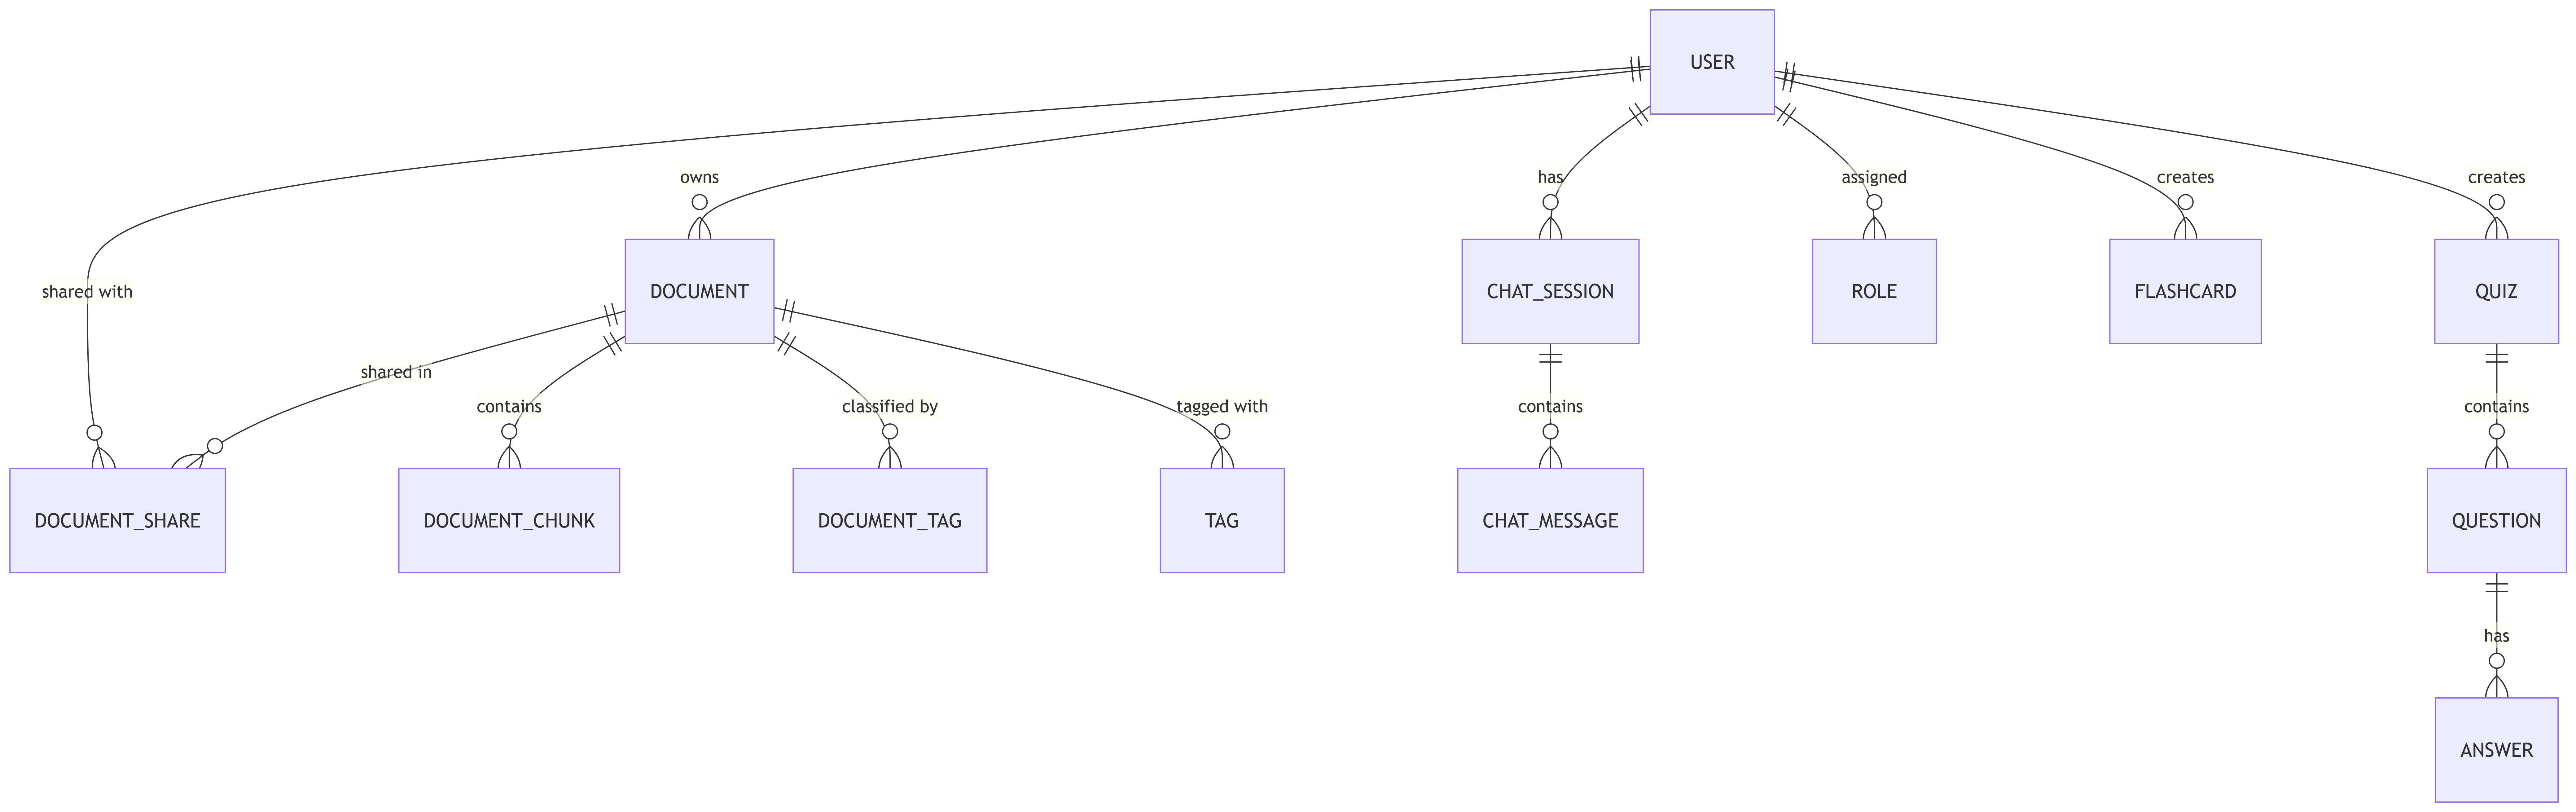
\includegraphics[width=\textwidth]{img/database_erd_no_at.png}
    \caption{Entity Relationship Diagram(ohne Attribute) des EduShelf Backends}
    \label{fig:erd}
\end{figure}
